\documentclass[journal,12pt,twocolumn]{IEEEtran}

\usepackage{amssymb}
\usepackage[cmex10]{amsmath}
\usepackage{amsthm}
\usepackage[export]{adjustbox}
\usepackage{bm}
\usepackage{tfrupee}
\usepackage{enumitem}

\newcommand{\myvec}[1]{\ensuremath{\begin{pmatrix}#1\end{pmatrix}}}

\let\vec\mathbf

\begin{document}

\title{AI1103 ASSIGNMENT-2}
\author{DASARI SRINITH \\\vspace*{20pt} \Large ICSE 2019 Grade 12}
\maketitle


\textbf{Question 22:}

A carpenter has 90 ,80 and 50 running feet respectively of teak wood, plywood and rosewood which is used to produce product A and product B.
Each unit of product A requires 2, 1 and 1 running feet and each unit of product B requires 1, 2 and 1 running feet of teak wood,plywood and rosewood respectively. 
If product A is sold for \rupee~$48$ per unit and product B is sold for \rupee~$40$ per unit,
how many units of product A and product B should be produced and sold by the carpenter, in order to obtain the maximum gross income?

Formulate the above as a Linear Programming Problem and solve it, indicating clearly the feasible region in the graph.

\textbf{Solution:}

Let $x$ be the number of units of product A produced and $y$ be the number of units of product B produced and $I$ be the maximum gross income.
From the given information, the problem can be formulated as
\begin{align}
    I = \max_{x,y} 48x + 40y
    \\
    2x + y \le 90 
    \\
    x + 2y \le 80 
    \\
    x + y \le 50 
\end{align}
which can be expressed in vector form as
\begin{align}
    P = \max_{\vec{x}}\myvec{48 & 40}\vec{x}
    \\
    \myvec{2 & 1 \\ 1 & 2 \\ 1 & 1} \vec{x} \preceq \myvec{90 \\ 80 \\ 50}
    \\
    \vec{x} \succeq \vec{0}
\end{align}
\begin{enumerate}
    \item {\em Graphical solution:}
    
        From the Fig.1,
        \begin{figure}[ht]
	        \centering
	        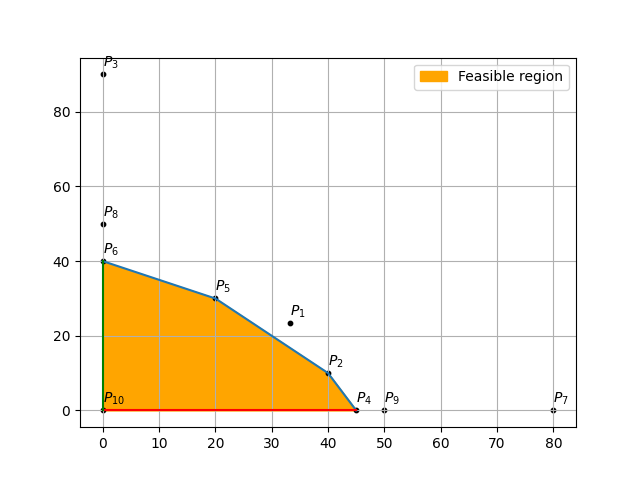
\includegraphics[width=\columnwidth]{plot2.png}
	        \caption{$P_6P_5P_2P_4P_{10}$ is the feasible region}
	        \label{fig}
        \end{figure}
        the feasible region is a pentagon with vertices
        \begin{align}
            \myvec{0 \\ 0},
            \myvec{45 \\ 0},
            \myvec{40 \\ 10},
            \myvec{20 \\ 30},
            \myvec{0 \\ 40}
        \end{align}
        with respective gross income
        \begin{align}
        	\myvec{48 & 40}\myvec{0 \\ 0} &= 0 \\
        	\myvec{48 & 40}\myvec{45 \\ 0} &= 2160 \\
        	\myvec{48 & 40}\myvec{40 \\ 10} &= 2320 \\
        	\myvec{48 & 40}\myvec{20 \\ 30} &= 2160 \\
        	\myvec{48 & 40}\myvec{0 \\ 40} &= 1600 
        \end{align}
        Thus, the carpenter should produce 40 units of product A and 10 units of product B for maximum gross income.
    \item {\em Lagrange Multipliers: }
    
        The given problem is expressed in the form 
        \begin{align}
	        P = -\min_{\vec{x}}\myvec{48 & 40}\vec{x} \\
	        \myvec{2 & 1 \\ 1 & 2 \\ 1 & 1 \\ -1 & 0 \\ 0 & -1} \vec{x}\preceq \myvec{90 \\ 80 \\50 \\ 0 \\0}
        \end{align}
        The Lagrangian, defined as the linear combination of the loss function and the constraints is defined as
        \begin{multline}
	        L\left({\vec{x},\bm{\lambda}}\right) =-\myvec{48 & 40}\vec{x} \\
	        + \lambda_1\left[{\myvec{2 & 1}\vec{x}-90}\right] \\
    	    + \lambda_2\left[{\myvec{1 & 2}\vec{x}-80}\right]
    	    + \lambda_3\left[{\myvec{1 & 1}\vec{x}-50}\right] \\
            + \lambda_4\left[{\myvec{-1 & 0}\vec{x}}\right] \\
            + \lambda_5\left[{\myvec{0 & -1}\vec{x}}\right]
        \end{multline}
        Taking the derivative
        \begin{align}
	        {\nabla L\left({\vec{x},\bm{\lambda}}\right)} = 0,
        \end{align}
        we obtain 
        \begin{align}
        	2\lambda_1 + \lambda_2 + \lambda_3 - \lambda_4 &= 48 \\
        	\lambda_1 + 2\lambda_2 + \lambda_3 - \lambda_5 &= 40 \\
        	2x_1 + x_2 &= 90 \\
        	x_1 + 2x_2 &= 80 \\
        	x_1 + x_2 &= 50 \\
        	x_1 &= 0 \\
        	x_2 &= 0
        \end{align}
        It is obvious that $x_1=0, x_2=0$ are infeasible.  Hence, considering $\lambda_4, \lambda_5$ as the inactive multipliers, And also from equations (20),(21),(22) we will not get unique values of $x_1$ and $x_2$ . So, there has to be a inactive multiplier in  $\lambda_1, \lambda_2$ and $\lambda_3$ .

        On solving equations (18) and (19) we get 
        \begin{align}
        	\lambda_1 - \lambda_2  &= 8 
        \end{align}
        From which we can imply that $\lambda_1$ can't be the inactive multiplier , because if it is then we get the value for $\lambda_2$ as a negative value .

        So , either $\lambda_2$ or $\lambda_3$ is the inactive multiplier.
        \begin{enumerate}
        \item {\em $\lambda_3$ is inactive multiplier:}
    
        So, considering $\lambda_1$ and $\lambda_2$ as active multipliers, the equations from (18) to (24) can be expressed as

        \begin{align}
            \myvec{0 & 0 & 2 & 1 \\
        		   0 & 0 & 1 & 2 \\
        		   2 & 1 & 0 & 0 \\
        		   1 & 2 & 0 & 0 }
        	\myvec{\vec{x} \\ \bm{\lambda}} = \myvec{48\\40\\90\\80}
        \end{align}
        yielding the solution as
        \begin{align}
	        \myvec{\vec{x} \\ \bm{\lambda}} = \myvec{100/3\\70/3\\56/3\\32/3}
        \end{align}
        But , the solution does not satisfy the constraint (4) , so this is not the correct case.
        \item {\em $\lambda_2$ is inactive multiplier:}
    
        So, considering $\lambda_1$ and $\lambda_3$ as active multipliers, the equations from (18) to (24) can be expressed as

        \begin{align}
            \myvec{0 & 0 & 2 & 1 \\
        		   0 & 0 & 1 & 1 \\
        		   2 & 1 & 0 & 0 \\
        		   1 & 1 & 0 & 0 }
        	\myvec{\vec{x} \\ \bm{\lambda}} = \myvec{48\\40\\90\\50}
        \end{align}
        yielding the solution as
        \begin{align}
        	\myvec{\vec{x} \\ \bm{\lambda}} = \myvec{40\\10\\8\\32}
        \end{align}
        This solution satisfies all the constraints , so we can say this is the optimal solution i.e,
        \begin{align}
        	\vec{x} = \myvec{40\\10}
        \end{align}
        \end{enumerate}

        The number of product A and product B should be produced and sold by carpenter , in order to obtain the maximum gross income are 40 and 10 respectively.

\end{enumerate}

\end{document}
